\documentclass{beamer}
\usepackage[utf8]{inputenc}
\usepackage{tikz}
\usepackage{pgfplots}
\usepackage{pgfplotstable}
\usepackage{forest}
\usepackage{istgame}
\usepackage{animate}
\usepackage{amsmath}
\usepackage{amsfonts}
\usepackage{amssymb}

% Configure pgfplots
\pgfplotsset{compat=1.18}

% TikZ libraries
\usetikzlibrary{calc,decorations.pathmorphing,3d,matrix,arrows.meta,positioning,shapes.geometric,angles,quotes,patterns,fillbetween}

% Theme
\usetheme{Madrid}
\usecolortheme{default}

\title{TikZ and PGFPlots Showcase}
\subtitle{Comprehensive Examples of Advanced Graphics in LaTeX}
\author{LaTeX Research Toolkit}
\date{\today}

\begin{document}

\frame{\titlepage}

% ===========================================
% BASIC DRAWING SECTION
% ===========================================

\begin{frame}{Basic Lines and Points}
\begin{center}
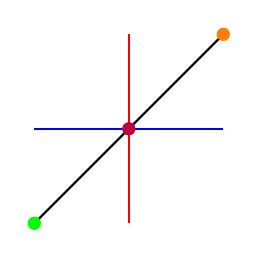
\begin{tikzpicture}[scale=1.2]
    \draw[thick] (0,0) -- (2,2);
    \draw[red, thick] (1,0) -- (1,2);
    \draw[blue, thick] (0,1) -- (2,1);
    \fill[green] (0,0) circle (2pt);
    \fill[orange] (2,2) circle (2pt);
    \fill[purple] (1,1) circle (2pt);
\end{tikzpicture}
\end{center}

\footnotesize
\texttt{\textbackslash draw[thick] (0,0) -- (2,2);}\\
\texttt{\textbackslash fill[green] (0,0) circle (2pt);}
\end{frame}

\begin{frame}{Grid and Coordinate System}
\begin{center}
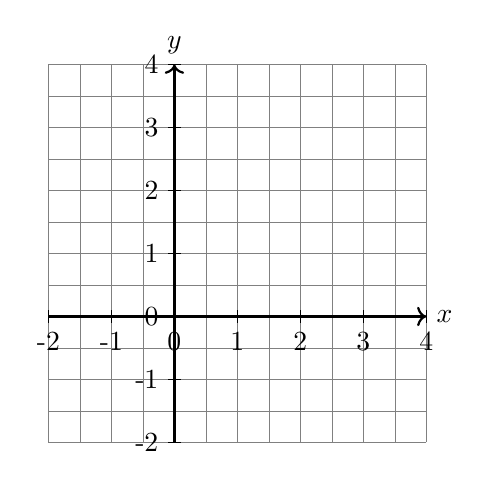
\begin{tikzpicture}[scale=0.8]
    \draw[step=0.5, gray, very thin] (-2,-2) grid (4,4);
    \draw[thick, ->] (-2,0) -- (4,0) node[right] {$x$};
    \draw[thick, ->] (0,-2) -- (0,4) node[above] {$y$};
    \foreach \x in {-2,-1,0,1,2,3,4}
        \draw (\x,0.1) -- (\x,-0.1) node[below] {\x};
    \foreach \y in {-2,-1,0,1,2,3,4}
        \draw (0.1,\y) -- (-0.1,\y) node[left] {\y};
\end{tikzpicture}
\end{center}

\footnotesize
\texttt{\textbackslash draw[step=0.5, gray, very thin] (-2,-2) grid (4,4);}
\end{frame}

\begin{frame}{Basic Shapes}
\begin{center}
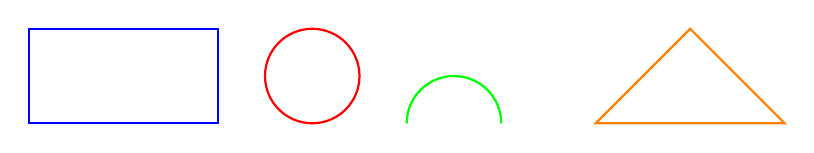
\begin{tikzpicture}[scale=1.2]
    \draw[blue, thick] (0,0) rectangle (2,1);
    \draw[red, thick] (3,0.5) circle (0.5);
    \draw[green, thick] (5,0) arc (0:180:0.5);
    \draw[orange, thick] (6,0) -- (7,1) -- (8,0) -- cycle;
\end{tikzpicture}
\end{center}

\footnotesize
\texttt{\textbackslash draw[blue, thick] (0,0) rectangle (2,1);}\\
\texttt{\textbackslash draw[red, thick] (3,0.5) circle (0.5);}
\end{frame}

% ===========================================
% 2D SHAPES AND ARCS SECTION
% ===========================================

\begin{frame}{Rectangles with Different Styles}
\begin{center}
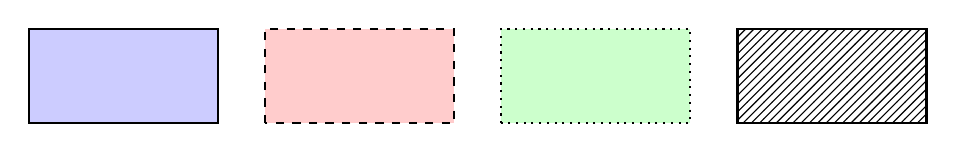
\begin{tikzpicture}[scale=1.2]
    \draw[thick, fill=blue!20] (0,0) rectangle (2,1);
    \draw[thick, fill=red!20, dashed] (2.5,0) rectangle (4.5,1);
    \draw[thick, fill=green!20, dotted] (5,0) rectangle (7,1);
    \draw[thick, fill=orange!20, pattern=north east lines] (7.5,0) rectangle (9.5,1);
\end{tikzpicture}
\end{center}

\footnotesize
\texttt{\textbackslash draw[thick, fill=blue!20] (0,0) rectangle (2,1);}\\
\texttt{\textbackslash draw[thick, fill=red!20, dashed] (2.5,0) rectangle (4.5,1);}
\end{frame}

\begin{frame}{Circles and Ellipses}
\begin{center}
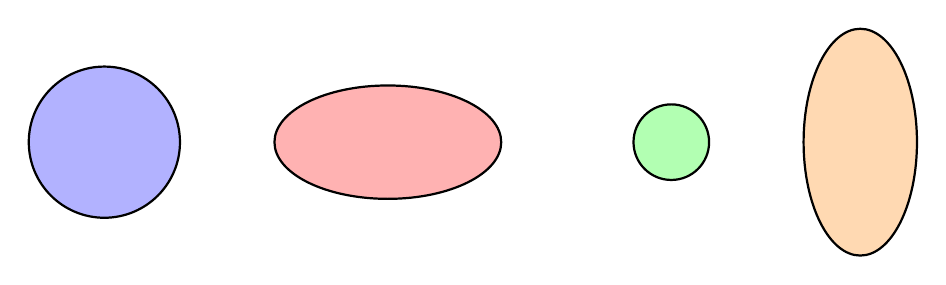
\begin{tikzpicture}[scale=1.2]
    \draw[thick, fill=blue!30] (0,0) circle (0.8);
    \draw[thick, fill=red!30] (3,0) ellipse (1.2 and 0.6);
    \draw[thick, fill=green!30] (6,0) circle (0.4);
    \draw[thick, fill=orange!30] (8,0) ellipse (0.6 and 1.2);
\end{tikzpicture}
\end{center}

\footnotesize
\texttt{\textbackslash draw[thick, fill=blue!30] (0,0) circle (0.8);}\\
\texttt{\textbackslash draw[thick, fill=red!30] (3,0) ellipse (1.2 and 0.6);}
\end{frame}

\begin{frame}{Arcs and Curves}
\begin{center}
\begin{tikzpicture}[scale=1.2]
    \draw[thick, blue] (0,0) arc (0:90:1);
    \draw[thick, red] (2,0) arc (0:180:1);
    \draw[thick, green] (4,0) arc (0:270:1);
    \draw[thick, orange] (6,0) .. controls (7,1) and (8,1) .. (9,0);
\end{tikzpicture}
\end{center}

\footnotesize
\texttt{\textbackslash draw[thick, blue] (0,0) arc (0:90:1);}\\
\texttt{\textbackslash draw[thick, orange] (6,0) .. controls (7,1) and (8,1) .. (9,0);}
\end{frame}

% ===========================================
% TRIANGLES SECTION
% ===========================================

\begin{frame}{Labeled Triangle}
\begin{center}
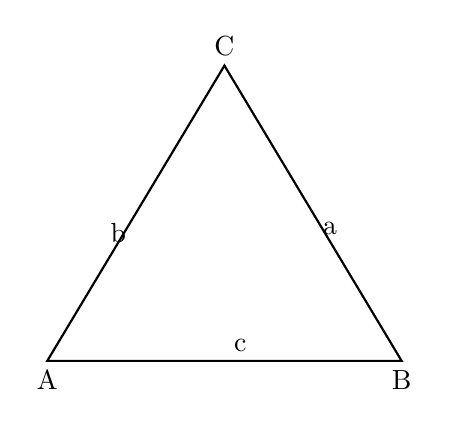
\begin{tikzpicture}[scale=1.5]
    \draw[thick] (0,0) -- (3,0) -- (1.5,2.5) -- cycle;
    \node[below] at (0,0) {A};
    \node[below] at (3,0) {B};
    \node[above] at (1.5,2.5) {C};
    \node[above right] at (1.5,0) {c};
    \node[below left] at (0.75,1.25) {b};
    \node[below right] at (2.25,1.25) {a};
\end{tikzpicture}
\end{center}

\footnotesize
\texttt{\textbackslash draw[thick] (0,0) -- (3,0) -- (1.5,2.5) -- cycle;}\\
\texttt{\textbackslash node[below] at (0,0) \{A\};}
\end{frame}

\begin{frame}{Triangle with Angle Marks}
\begin{center}
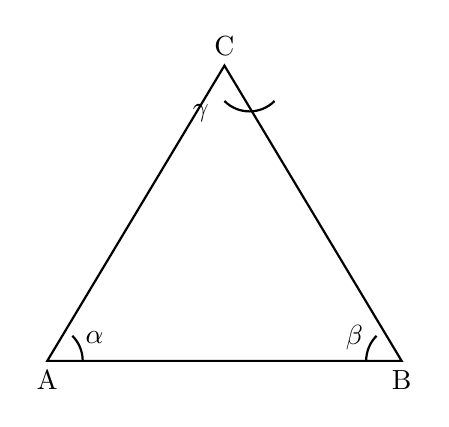
\begin{tikzpicture}[scale=1.5]
    \draw[thick] (0,0) -- (3,0) -- (1.5,2.5) -- cycle;
    \node[below] at (0,0) {A};
    \node[below] at (3,0) {B};
    \node[above] at (1.5,2.5) {C};
    
    % Angle marks
    \draw[thick] (0.3,0) arc (0:45:0.3);
    \node at (0.4,0.2) {$\alpha$};
    
    \draw[thick] (2.7,0) arc (180:135:0.3);
    \node at (2.6,0.2) {$\beta$};
    
    \draw[thick] (1.5,2.2) arc (225:315:0.3);
    \node at (1.3,2.1) {$\gamma$};
\end{tikzpicture}
\end{center}

\footnotesize
\texttt{\textbackslash draw[thick] (0.3,0) arc (0:45:0.3);}\\
\texttt{\textbackslash node at (0.4,0.2) \{\$\textbackslash alpha\$\};}
\end{frame}

\begin{frame}{Right Triangle with Measurements}
\begin{center}
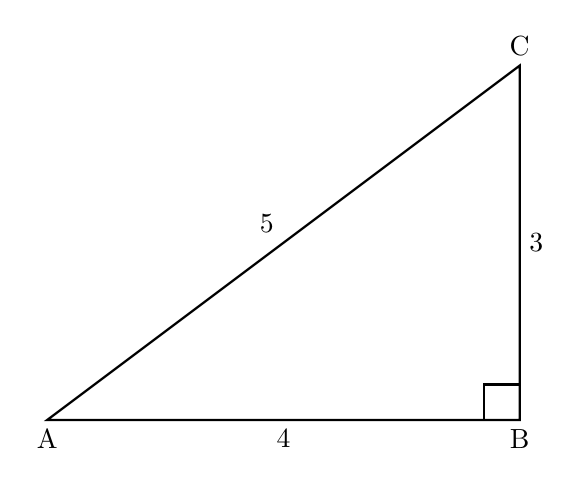
\begin{tikzpicture}[scale=1.5]
    \draw[thick] (0,0) -- (4,0) -- (4,3) -- cycle;
    \node[below] at (0,0) {A};
    \node[below] at (4,0) {B};
    \node[above] at (4,3) {C};
    
    % Right angle mark
    \draw[thick] (3.7,0) -- (3.7,0.3) -- (4,0.3);
    
    % Side lengths
    \node[below] at (2,0) {4};
    \node[right] at (4,1.5) {3};
    \node[above left] at (2,1.5) {5};
\end{tikzpicture}
\end{center}

\footnotesize
\texttt{\textbackslash draw[thick] (3.7,0) -- (3.7,0.3) -- (4,0.3);}
\end{frame}

% ===========================================
% VENN DIAGRAMS SECTION
% ===========================================

\begin{frame}{Two-Set Venn Diagram}
\begin{center}
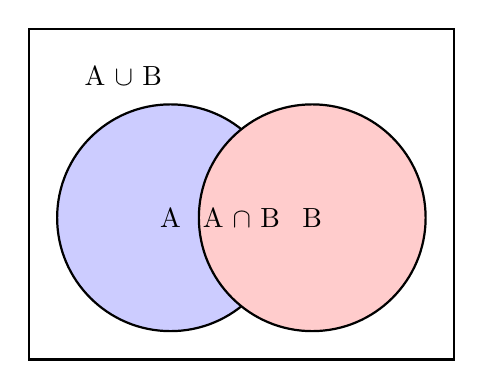
\begin{tikzpicture}[scale=1.2]
    \draw[thick, fill=blue!20] (0,0) circle (1.2);
    \draw[thick, fill=red!20] (1.5,0) circle (1.2);
    \draw[thick] (-1.5,-1.5) rectangle (3,2);
    
    \node at (0,0) {A};
    \node at (1.5,0) {B};
    \node at (0.75,0) {A $\cap$ B};
    \node at (-0.5,1.5) {A $\cup$ B};
\end{tikzpicture}
\end{center}

\footnotesize
\texttt{\textbackslash draw[thick, fill=blue!20] (0,0) circle (1.2);}\\
\texttt{\textbackslash draw[thick, fill=red!20] (1.5,0) circle (1.2);}
\end{frame}

\begin{frame}{Three-Set Venn Diagram}
\begin{center}
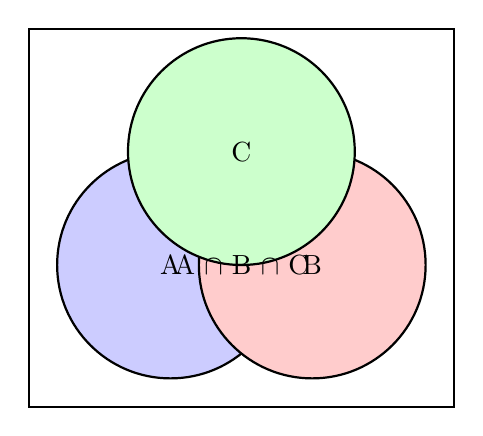
\begin{tikzpicture}[scale=1.2]
    \draw[thick, fill=blue!20] (0,0) circle (1.2);
    \draw[thick, fill=red!20] (1.5,0) circle (1.2);
    \draw[thick, fill=green!20] (0.75,1.2) circle (1.2);
    \draw[thick] (-1.5,-1.5) rectangle (3,2.5);
    
    \node at (0,0) {A};
    \node at (1.5,0) {B};
    \node at (0.75,1.2) {C};
    \node at (0.75,0) {A $\cap$ B $\cap$ C};
\end{tikzpicture}
\end{center}

\footnotesize
\texttt{\textbackslash draw[thick, fill=green!20] (0.75,1.2) circle (1.2);}
\end{frame}

% ===========================================
% PROBABILITY TREES SECTION
% ===========================================

\begin{frame}{Simple Probability Tree}
\begin{center}
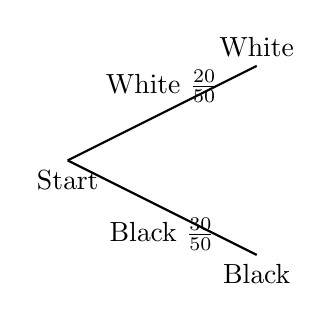
\begin{tikzpicture}[scale=1.2]
    \coordinate (A) at (0,0);
    \coordinate (B) at (2,1);
    \coordinate (C) at (2,-1);
    
    \draw[thick] (A) -- node[above] {White $\frac{20}{50}$} (B);
    \draw[thick] (A) -- node[below] {Black $\frac{30}{50}$} (C);
    
    \node[below] at (A) {Start};
    \node[above] at (B) {White};
    \node[below] at (C) {Black};
\end{tikzpicture}
\end{center}

\footnotesize
\texttt{\textbackslash draw[thick] (A) -- node[above] \{White \$\textbackslash frac\{20\}\{50\}\$\} (B);}
\end{frame}

\begin{frame}{Two-Stage Probability Tree}
\begin{center}
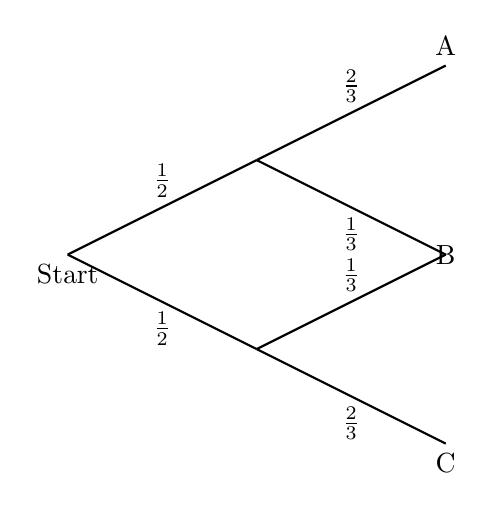
\begin{tikzpicture}[scale=1.2]
    \coordinate (A) at (0,0);
    \coordinate (B) at (2,1);
    \coordinate (C) at (2,-1);
    \coordinate (D) at (4,2);
    \coordinate (E) at (4,0);
    \coordinate (F) at (4,-2);
    
    \draw[thick] (A) -- node[above] {$\frac{1}{2}$} (B);
    \draw[thick] (A) -- node[below] {$\frac{1}{2}$} (C);
    \draw[thick] (B) -- node[above] {$\frac{2}{3}$} (D);
    \draw[thick] (B) -- node[below] {$\frac{1}{3}$} (E);
    \draw[thick] (C) -- node[above] {$\frac{1}{3}$} (E);
    \draw[thick] (C) -- node[below] {$\frac{2}{3}$} (F);
    
    \node[below] at (A) {Start};
    \node[above] at (D) {A};
    \node at (E) {B};
    \node[below] at (F) {C};
\end{tikzpicture}
\end{center}

\footnotesize
Two-stage decision tree with probability labels
\end{frame}

% ===========================================
% BASIC PLOTTING SECTION
% ===========================================

\begin{frame}{Simple Function Plot}
\begin{center}
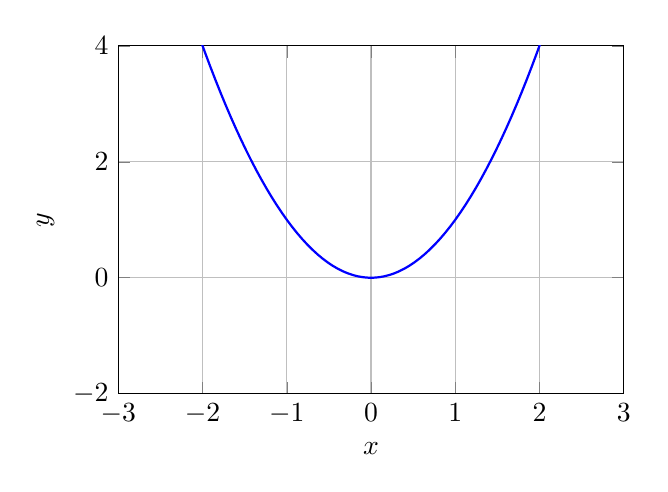
\begin{tikzpicture}
\begin{axis}[
    xlabel={$x$},
    ylabel={$y$},
    grid=both,
    xmin=-3, xmax=3,
    ymin=-2, ymax=4,
    width=8cm,
    height=6cm
]
\addplot[thick, blue, domain=-3:3, samples=100] {x^2};
\end{axis}
\end{tikzpicture}
\end{center}

\footnotesize
\texttt{\textbackslash addplot[thick, blue, domain=-3:3, samples=100] \{x\textasciicircum 2\};}
\end{frame}

\begin{frame}{Multiple Function Plots}
\begin{center}
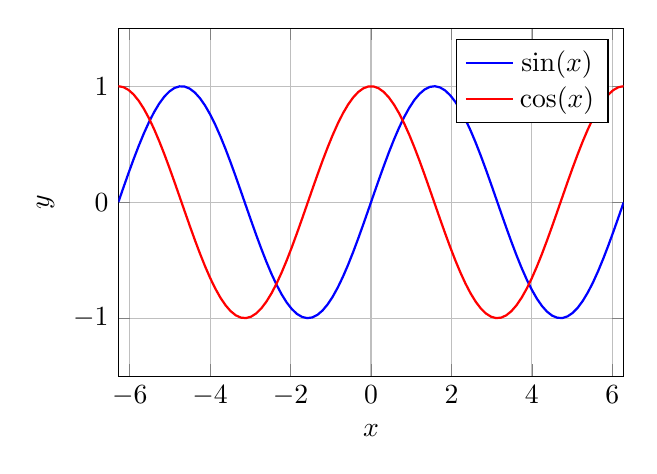
\begin{tikzpicture}
\begin{axis}[
    xlabel={$x$},
    ylabel={$y$},
    grid=both,
    xmin=-2*pi, xmax=2*pi,
    ymin=-1.5, ymax=1.5,
    width=8cm,
    height=6cm,
    legend pos=north east
]
\addplot[thick, blue, domain=-2*pi:2*pi, samples=100] {sin(deg(x))};
\addplot[thick, red, domain=-2*pi:2*pi, samples=100] {cos(deg(x))};
\legend{$\sin(x)$, $\cos(x)$}
\end{axis}
\end{tikzpicture}
\end{center}

\footnotesize
\texttt{\textbackslash addplot[thick, blue] \{sin(deg(x))\};}\\
\texttt{\textbackslash legend\{\$\textbackslash sin(x)\$, \$\textbackslash cos(x)\$\}}
\end{frame}

\begin{frame}{Area Under Curve}
\begin{center}
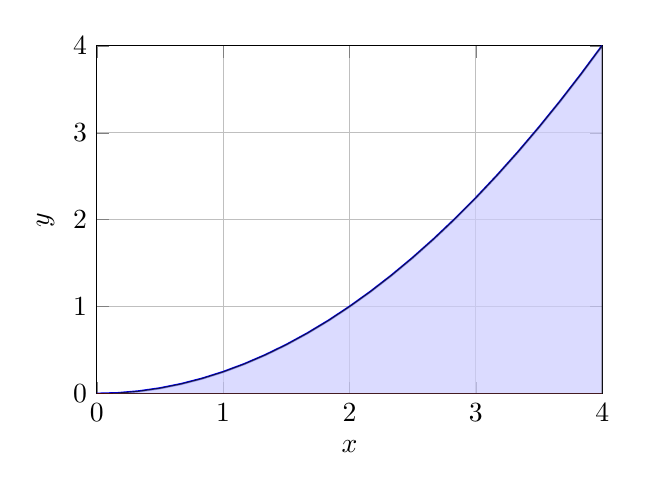
\begin{tikzpicture}
\begin{axis}[
    xlabel={$x$},
    ylabel={$y$},
    grid=both,
    xmin=0, xmax=4,
    ymin=0, ymax=4,
    width=8cm,
    height=6cm
]
\addplot[thick, blue, domain=0:4] {x^2/4};
\addplot[thick, red, domain=0:4] {0};
\addplot[fill=blue!20, opacity=0.7, domain=0:4] {x^2/4} \closedcycle;
\end{axis}
\end{tikzpicture}
\end{center}

\footnotesize
\texttt{\textbackslash addplot[fill=blue!20, opacity=0.7] fill between[of=A and B];}
\end{frame}

% ===========================================
% ADVANCED PLOTTING SECTION
% ===========================================

\begin{frame}{Exponential and Logarithmic Functions}
\begin{center}
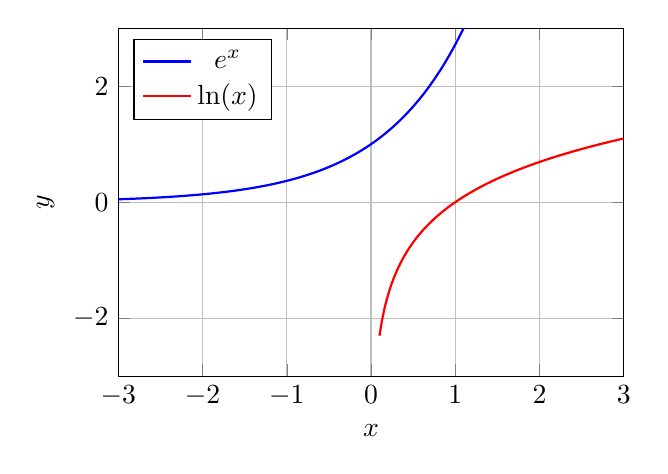
\begin{tikzpicture}
\begin{axis}[
    xlabel={$x$},
    ylabel={$y$},
    grid=both,
    xmin=-3, xmax=3,
    ymin=-3, ymax=3,
    width=8cm,
    height=6cm,
    legend pos=north west
]
\addplot[thick, blue, domain=-3:3, samples=100] {exp(x)};
\addplot[thick, red, domain=0.1:3, samples=100] {ln(x)};
\legend{$e^x$, $\ln(x)$}
\end{axis}
\end{tikzpicture}
\end{center}

\footnotesize
\texttt{\textbackslash addplot[thick, blue] \{exp(x)\};}\\
\texttt{\textbackslash addplot[thick, red] \{ln(x)\};}
\end{frame}

\begin{frame}{Parametric Curves}
\begin{center}
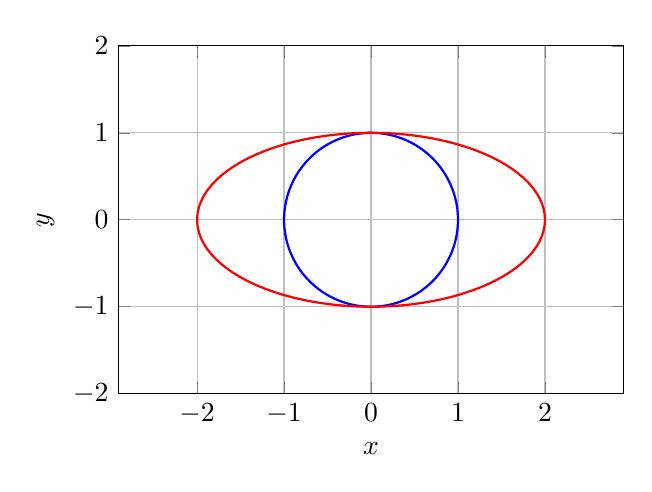
\begin{tikzpicture}
\begin{axis}[
    xlabel={$x$},
    ylabel={$y$},
    grid=both,
    xmin=-2, xmax=2,
    ymin=-2, ymax=2,
    width=8cm,
    height=6cm,
    axis equal
]
\addplot[thick, blue, domain=0:2*pi, samples=100] ({cos(deg(x))}, {sin(deg(x))});
\addplot[thick, red, domain=0:2*pi, samples=100] ({2*cos(deg(x))}, {sin(deg(x))});
\end{axis}
\end{tikzpicture}
\end{center}

\footnotesize
\texttt{\textbackslash addplot[thick, blue] (\{cos(deg(x))\}, \{sin(deg(x))\})}
\end{frame}

\begin{frame}{Scatter Plot with Data Points}
\begin{center}
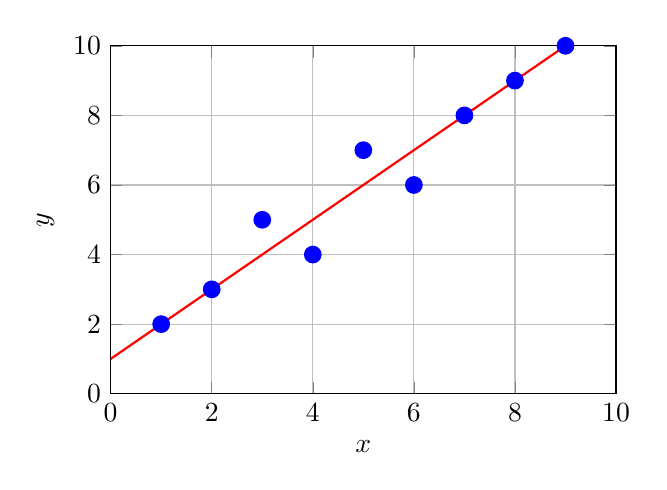
\begin{tikzpicture}
\begin{axis}[
    xlabel={$x$},
    ylabel={$y$},
    grid=both,
    xmin=0, xmax=10,
    ymin=0, ymax=10,
    width=8cm,
    height=6cm
]
\addplot[only marks, mark=*, mark size=3pt, blue] coordinates {
    (1,2) (2,3) (3,5) (4,4) (5,7) (6,6) (7,8) (8,9) (9,10)
};
\addplot[thick, red, domain=0:10] {x + 1};
\end{axis}
\end{tikzpicture}
\end{center}

\footnotesize
\texttt{\textbackslash addplot[only marks, mark=*, mark size=3pt, blue] coordinates \{\}}
\end{frame}

% ===========================================
% SHADING BETWEEN CURVES SECTION
% ===========================================

\begin{frame}{Area Between Two Curves}
\begin{center}
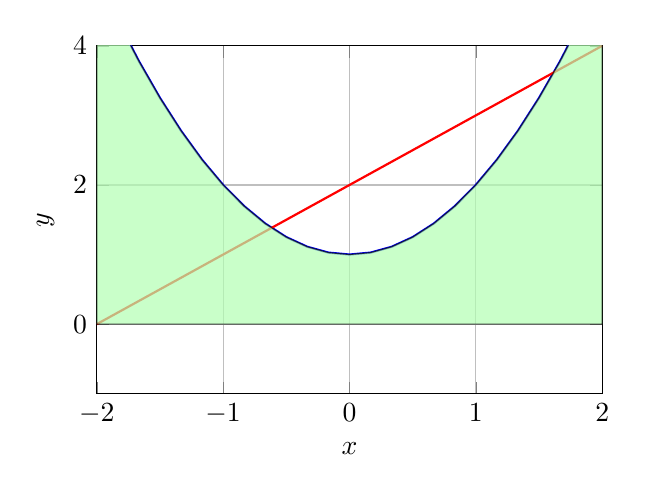
\begin{tikzpicture}
\begin{axis}[
    xlabel={$x$},
    ylabel={$y$},
    grid=both,
    xmin=-2, xmax=2,
    ymin=-1, ymax=4,
    width=8cm,
    height=6cm
]
\addplot[thick, blue, domain=-2:2] {x^2 + 1};
\addplot[thick, red, domain=-2:2] {x + 2};
\addplot[fill=green!30, opacity=0.7, domain=-2:2] {x^2 + 1} \closedcycle;
\end{axis}
\end{tikzpicture}
\end{center}

\footnotesize
\texttt{\textbackslash addplot[fill=green!30, opacity=0.7] fill between[of=A and B];}
\end{frame}

\begin{frame}{Multiple Shaded Regions}
\begin{center}
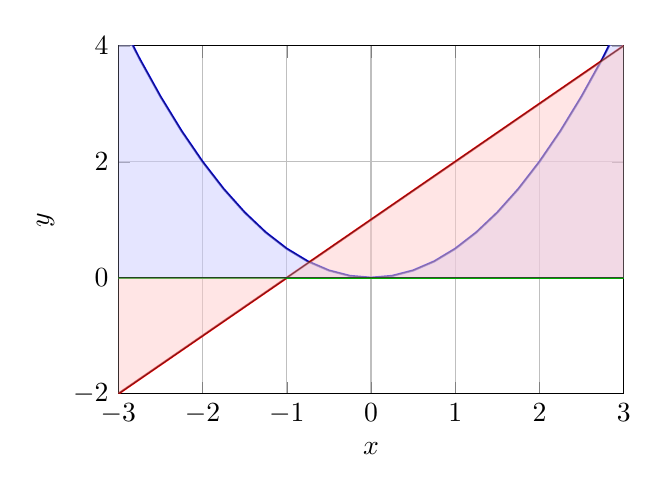
\begin{tikzpicture}
\begin{axis}[
    xlabel={$x$},
    ylabel={$y$},
    grid=both,
    xmin=-3, xmax=3,
    ymin=-2, ymax=4,
    width=8cm,
    height=6cm
]
\addplot[thick, blue, domain=-3:3] {x^2/2};
\addplot[thick, red, domain=-3:3] {x + 1};
\addplot[thick, green, domain=-3:3] {0};
\addplot[fill=blue!20, opacity=0.5, domain=-3:3] {x^2/2} \closedcycle;
\addplot[fill=red!20, opacity=0.5, domain=-3:3] {x + 1} \closedcycle;
\end{axis}
\end{tikzpicture}
\end{center}

\footnotesize
Multiple shaded regions with different colors
\end{frame}

% ===========================================
% EXTERNAL DATA PLOTTING SECTION
% ===========================================

\begin{frame}{Data from CSV File}
\begin{center}
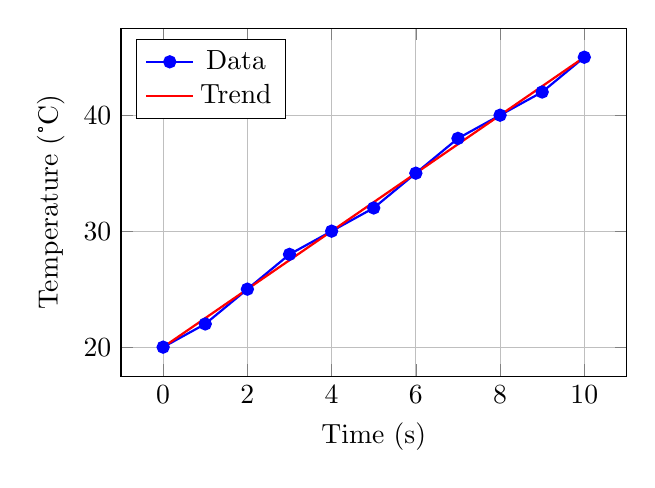
\begin{tikzpicture}
\begin{axis}[
    xlabel={Time (s)},
    ylabel={Temperature (°C)},
    grid=both,
    width=8cm,
    height=6cm,
    legend pos=north west
]
% Simulated data points
\addplot[thick, blue, mark=*, mark size=2pt] coordinates {
    (0,20) (1,22) (2,25) (3,28) (4,30) (5,32) (6,35) (7,38) (8,40) (9,42) (10,45)
};
\addplot[thick, red, domain=0:10] {20 + 2.5*x};
\legend{Data, Trend}
\end{axis}
\end{tikzpicture}
\end{center}

\footnotesize
\texttt{\textbackslash addplot[thick, blue, mark=*, mark size=2pt] coordinates \{\}}
\end{frame}

% ===========================================
% FLOWCHARTS SECTION
% ===========================================

\begin{frame}{Simple Flowchart}
\begin{center}
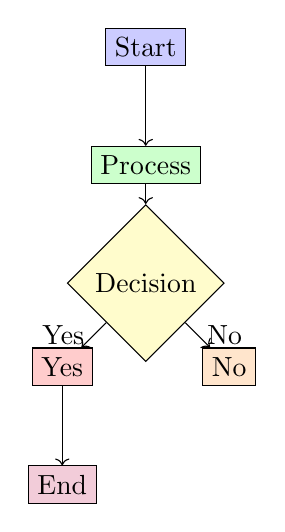
\begin{tikzpicture}[node distance=1.5cm]
    \node[rectangle, draw, fill=blue!20] (start) {Start};
    \node[rectangle, draw, fill=green!20, below of=start] (process) {Process};
    \node[diamond, draw, fill=yellow!20, below of=process] (decision) {Decision};
    \node[rectangle, draw, fill=red!20, below left of=decision] (yes) {Yes};
    \node[rectangle, draw, fill=orange!20, below right of=decision] (no) {No};
    \node[rectangle, draw, fill=purple!20, below of=yes] (end) {End};
    
    \draw[->] (start) -- (process);
    \draw[->] (process) -- (decision);
    \draw[->] (decision) -- node[left] {Yes} (yes);
    \draw[->] (decision) -- node[right] {No} (no);
    \draw[->] (yes) -- (end);
\end{tikzpicture}
\end{center}

\footnotesize
\texttt{\textbackslash node[diamond, draw, fill=yellow!20, below of=decision] \{decision\};}
\end{frame}

\begin{frame}{Complex Flowchart with Loops}
\begin{center}
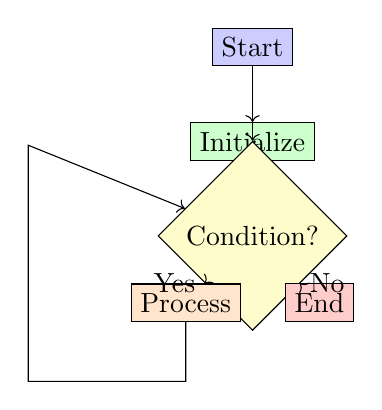
\begin{tikzpicture}[node distance=1.2cm]
    \node[rectangle, draw, fill=blue!20] (start) {Start};
    \node[rectangle, draw, fill=green!20, below of=start] (init) {Initialize};
    \node[diamond, draw, fill=yellow!20, below of=init] (condition) {Condition?};
    \node[rectangle, draw, fill=orange!20, below left of=condition] (process) {Process};
    \node[rectangle, draw, fill=red!20, below right of=condition] (end) {End};
    
    \draw[->] (start) -- (init);
    \draw[->] (init) -- (condition);
    \draw[->] (condition) -- node[left] {Yes} (process);
    \draw[->] (condition) -- node[right] {No} (end);
    \draw[->] (process) -- ++(0,-1) -- ++(-2,0) -- ++(0,3) -- (condition);
\end{tikzpicture}
\end{center}

\footnotesize
Loop structure with feedback arrow
\end{frame}

% ===========================================
% GEOMETRY FIGURES SECTION
% ===========================================

\begin{frame}{Annotated Circle}
\begin{center}
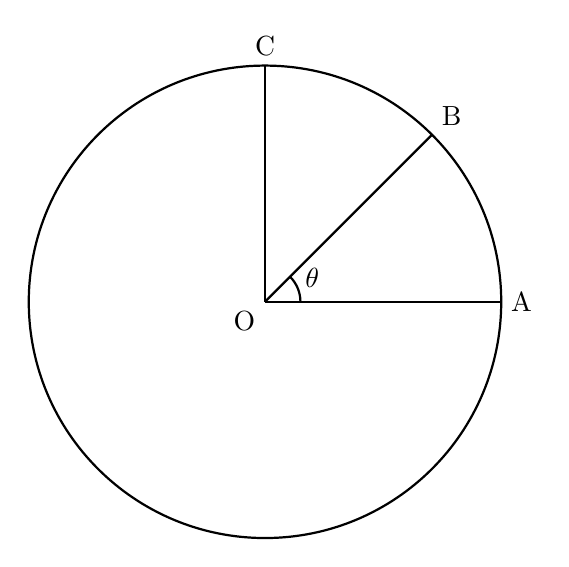
\begin{tikzpicture}[scale=1.5]
    \draw[thick] (0,0) circle (2);
    \draw[thick] (0,0) -- (2,0);
    \draw[thick] (0,0) -- (1.414,1.414);
    \draw[thick] (0,0) -- (0,2);
    
    \node at (0,0) [below left] {O};
    \node at (2,0) [right] {A};
    \node at (1.414,1.414) [above right] {B};
    \node at (0,2) [above] {C};
    
    \draw[thick] (0.3,0) arc (0:45:0.3);
    \node at (0.4,0.2) {$\theta$};
\end{tikzpicture}
\end{center}

\footnotesize
\texttt{\textbackslash draw[thick] (0,0) circle (2);}\\
\texttt{\textbackslash draw[thick] (0.3,0) arc (0:45:0.3);}
\end{frame}

\begin{frame}{Polygon with Measurements}
\begin{center}
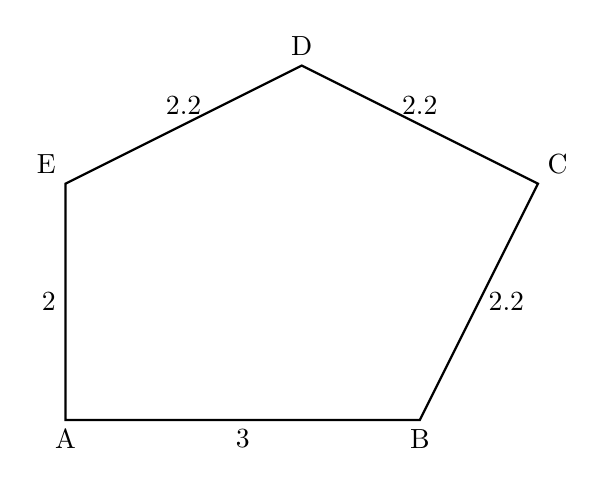
\begin{tikzpicture}[scale=1.5]
    \draw[thick] (0,0) -- (3,0) -- (4,2) -- (2,3) -- (0,2) -- cycle;
    \node[below] at (0,0) {A};
    \node[below] at (3,0) {B};
    \node[above right] at (4,2) {C};
    \node[above] at (2,3) {D};
    \node[above left] at (0,2) {E};
    
    % Side measurements
    \node[below] at (1.5,0) {3};
    \node[right] at (3.5,1) {2.2};
    \node[above] at (3,2.5) {2.2};
    \node[above] at (1,2.5) {2.2};
    \node[left] at (0,1) {2};
\end{tikzpicture}
\end{center}

\footnotesize
Irregular pentagon with labeled vertices and side lengths
\end{frame}

% ===========================================
% 3D PLOTS SECTION
% ===========================================

\begin{frame}{3D Surface Plot}
\begin{center}
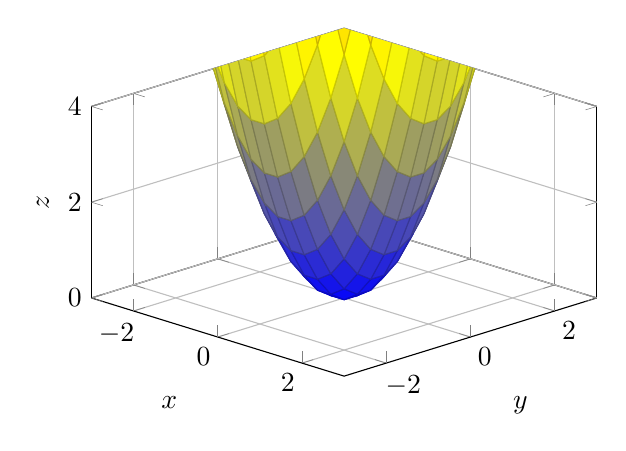
\begin{tikzpicture}
\begin{axis}[
    xlabel={$x$},
    ylabel={$y$},
    zlabel={$z$},
    grid=both,
    xmin=-3, xmax=3,
    ymin=-3, ymax=3,
    zmin=0, zmax=4,
    width=8cm,
    height=6cm,
    view={45}{30}
]
\addplot3[surf, domain=-3:3, samples=20] {x^2 + y^2};
\end{axis}
\end{tikzpicture}
\end{center}

\footnotesize
\texttt{\textbackslash addplot3[surf, domain=-3:3, samples=20] \{x\textasciicircum 2 + y\textasciicircum 2\};}
\end{frame}

\begin{frame}{3D Parametric Curve}
\begin{center}
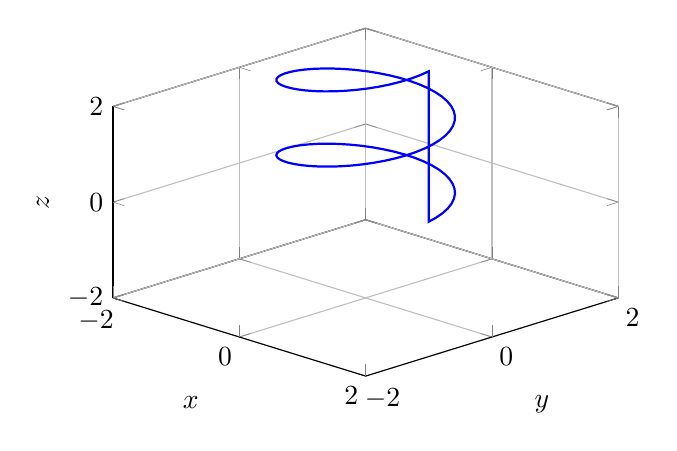
\begin{tikzpicture}
\begin{axis}[
    xlabel={$x$},
    ylabel={$y$},
    zlabel={$z$},
    grid=both,
    xmin=-2, xmax=2,
    ymin=-2, ymax=2,
    zmin=-2, zmax=2,
    width=8cm,
    height=6cm,
    view={45}{30}
]
\addplot3[thick, blue, domain=0:4*pi, samples=100] ({cos(deg(x))}, {sin(deg(x))}, {x/4});
\end{axis}
\end{tikzpicture}
\end{center}

\footnotesize
\texttt{\textbackslash addplot3[thick, blue] (\{cos(deg(x))\}, \{sin(deg(x))\}, \{x/4\})}
\end{frame}

% ===========================================
% ANIMATION SECTION
% ===========================================

\begin{frame}{Animated Function Plot}
\begin{center}
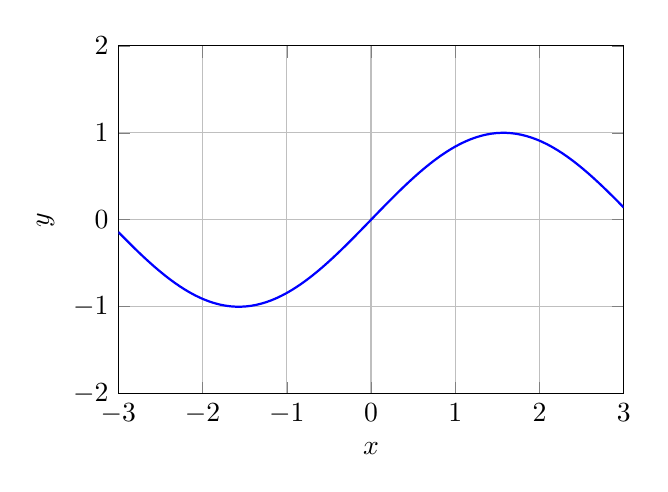
\begin{tikzpicture}
\begin{axis}[
    xlabel={$x$},
    ylabel={$y$},
    grid=both,
    xmin=-3, xmax=3,
    ymin=-2, ymax=2,
    width=8cm,
    height=6cm
]
\addplot[thick, blue, domain=-3:3, samples=100] {sin(deg(x))};
\end{axis}
\end{tikzpicture}
\end{center}

\footnotesize
Static version of animated plot (use animate package for motion)
\end{frame}

% ===========================================
% ADVANCED AXIS STYLING SECTION
% ===========================================

\begin{frame}{Logarithmic Scale}
\begin{center}
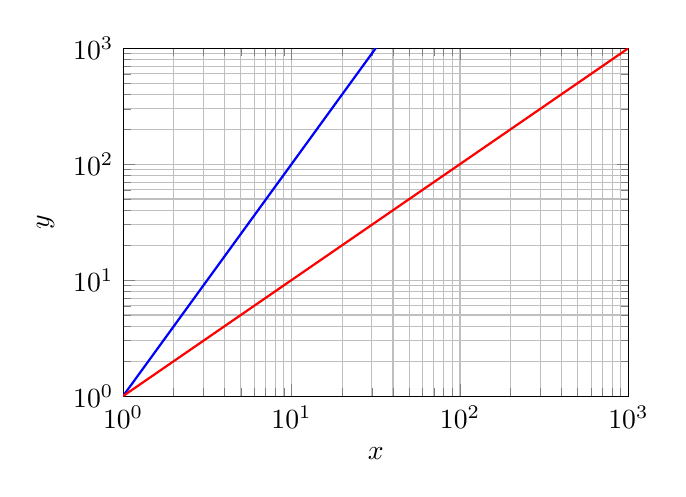
\begin{tikzpicture}
\begin{axis}[
    xlabel={$x$},
    ylabel={$y$},
    grid=both,
    xmin=1, xmax=1000,
    ymin=1, ymax=1000,
    width=8cm,
    height=6cm,
    xmode=log,
    ymode=log
]
\addplot[thick, blue, domain=1:1000, samples=100] {x^2};
\addplot[thick, red, domain=1:1000, samples=100] {x};
\end{axis}
\end{tikzpicture}
\end{center}

\footnotesize
\texttt{xmode=log, ymode=log}
\end{frame}

\begin{frame}{Custom Tick Marks}
\begin{center}
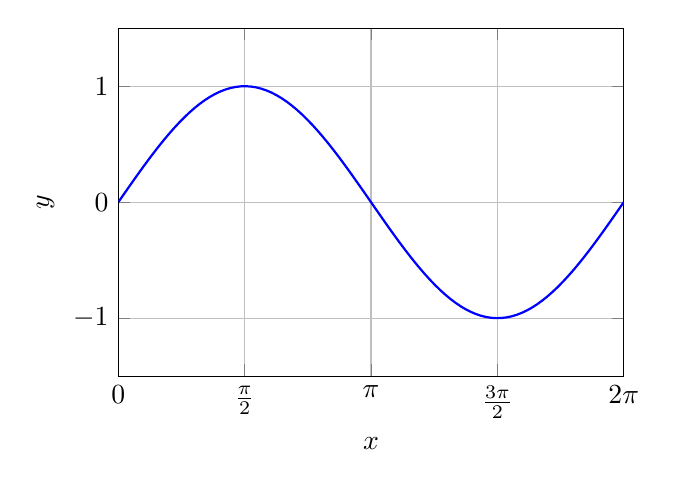
\begin{tikzpicture}
\begin{axis}[
    xlabel={$x$},
    ylabel={$y$},
    grid=both,
    xmin=0, xmax=2*pi,
    ymin=-1.5, ymax=1.5,
    width=8cm,
    height=6cm,
    xtick={0,pi/2,pi,3*pi/2,2*pi},
    xticklabels={0,$\frac{\pi}{2}$,$\pi$,$\frac{3\pi}{2}$,$2\pi$},
    ytick={-1,0,1}
]
\addplot[thick, blue, domain=0:2*pi, samples=100] {sin(deg(x))};
\end{axis}
\end{tikzpicture}
\end{center}

\footnotesize
\texttt{xtick=\{0,pi/2,pi,3*pi/2,2*pi\},}\\
\texttt{xticklabels=\{0,\$\textbackslash frac\{\textbackslash pi\}\{2\}\$,\$\textbackslash pi\$,\$\textbackslash frac\{3\textbackslash pi\}\{2\}\$,\$2\textbackslash pi\$\}}
\end{frame}

% ===========================================
% MATHEMATICAL DIAGRAMS SECTION
% ===========================================

\begin{frame}{State Machine}
\begin{center}
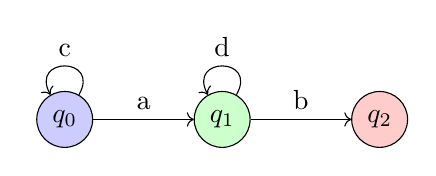
\begin{tikzpicture}[node distance=2cm]
    \node[circle, draw, fill=blue!20] (q0) {$q_0$};
    \node[circle, draw, fill=green!20, right of=q0] (q1) {$q_1$};
    \node[circle, draw, fill=red!20, right of=q1] (q2) {$q_2$};
    
    \draw[->] (q0) -- node[above] {a} (q1);
    \draw[->] (q1) -- node[above] {b} (q2);
    \draw[->] (q0) to[out=60,in=120,looseness=4] node[above] {c} (q0);
    \draw[->] (q1) to[out=60,in=120,looseness=4] node[above] {d} (q1);
\end{tikzpicture}
\end{center}

\footnotesize
\texttt{\textbackslash draw[->] (q0) to[out=60,in=120,looseness=4] node[above] \{c\} (q0);}
\end{frame}

\begin{frame}{Commutative Diagram}
\begin{center}
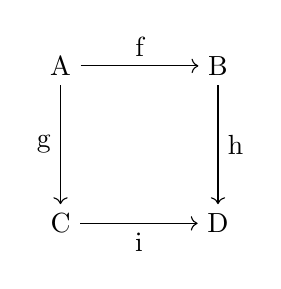
\begin{tikzpicture}[node distance=2cm]
    \node (A) {A};
    \node[right of=A] (B) {B};
    \node[below of=A] (C) {C};
    \node[below of=B] (D) {D};
    
    \draw[->] (A) -- node[above] {f} (B);
    \draw[->] (A) -- node[left] {g} (C);
    \draw[->] (B) -- node[right] {h} (D);
    \draw[->] (C) -- node[below] {i} (D);
\end{tikzpicture}
\end{center}

\footnotesize
\texttt{\textbackslash draw[->] (A) -- node[above] \{f\} (B);}
\end{frame}

% ===========================================
% TIKZ LIBRARIES SECTION
% ===========================================

\begin{frame}{Matrix of Nodes}
\begin{center}
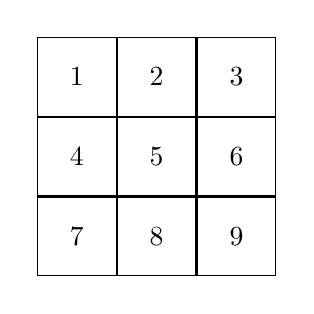
\begin{tikzpicture}
\matrix[matrix of nodes, nodes={draw, minimum size=1cm}] {
    1 & 2 & 3 \\
    4 & 5 & 6 \\
    7 & 8 & 9 \\
};
\end{tikzpicture}
\end{center}

\footnotesize
\texttt{\textbackslash matrix[matrix of nodes, nodes=\{draw, minimum size=1cm\}] \{\}}
\end{frame}

\begin{frame}{Decorative Paths}
\begin{center}
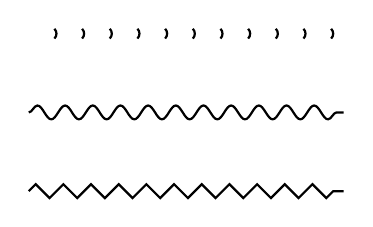
\begin{tikzpicture}
\draw[thick, decorate, decoration={zigzag}] (0,0) -- (4,0);
\draw[thick, decorate, decoration={snake}] (0,1) -- (4,1);
\draw[thick, decorate, decoration={waves}] (0,2) -- (4,2);
\end{tikzpicture}
\end{center}

\footnotesize
\texttt{\textbackslash draw[thick, decorate, decoration=\{zigzag\}] (0,0) -- (4,0);}
\end{frame}

\begin{frame}{3D Cube}
\begin{center}
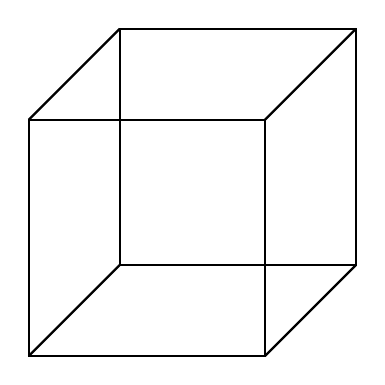
\begin{tikzpicture}[scale=1.5]
\draw[thick] (0,0,0) -- (2,0,0) -- (2,2,0) -- (0,2,0) -- cycle;
\draw[thick] (0,0,0) -- (0,0,2);
\draw[thick] (2,0,0) -- (2,0,2);
\draw[thick] (2,2,0) -- (2,2,2);
\draw[thick] (0,2,0) -- (0,2,2);
\draw[thick] (0,0,2) -- (2,0,2) -- (2,2,2) -- (0,2,2) -- cycle;
\end{tikzpicture}
\end{center}

\footnotesize
\texttt{\textbackslash draw[thick] (0,0,0) -- (2,0,0) -- (2,2,0) -- (0,2,0) -- cycle;}
\end{frame}

% ===========================================
% FOREST PACKAGE SECTION
% ===========================================

\begin{frame}{Tree with Forest Package}
\begin{center}
\begin{forest}
[Root
    [Child 1
        [Grandchild 1]
        [Grandchild 2]
    ]
    [Child 2
        [Grandchild 3]
    ]
    [Child 3]
]
\end{forest}
\end{center}

\footnotesize
\texttt{\textbackslash begin\{forest\}}\\
\texttt{[Root}\\
\texttt{    [Child 1]}
\end{frame}

% ===========================================
% ISTGAME PACKAGE SECTION
% ===========================================

\begin{frame}{Game Tree with istgame}
\begin{center}
\begin{istgame}
\xtdistance{15mm}{30mm}
\istroot(0){Player 1}
  \istb{L}[al] \istb{R}[ar]
  \endist
\istroot(1)(0-1){Player 2}
  \istb{l}[al] \istb{r}[ar]
  \endist
\istroot(2)(0-2){Player 2}
  \istb{l}[al] \istb{r}[ar]
  \endist
\end{istgame}
\end{center}

\footnotesize
\texttt{\textbackslash istroot(0)\{Player 1\}}\\
\texttt{\textbackslash istb\{L\}[al] \textbackslash istb\{R\}[ar]}
\end{frame}

% ===========================================
% ADVANCED EXAMPLES SECTION
% ===========================================

\begin{frame}{Neural Network Diagram}
\begin{center}
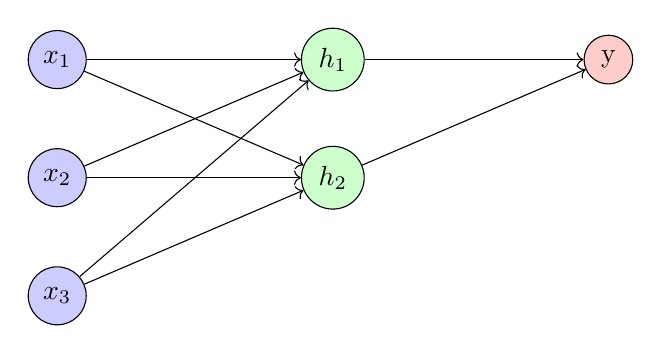
\begin{tikzpicture}[node distance=1.5cm]
    % Input layer
    \node[circle, draw, fill=blue!20] (i1) {$x_1$};
    \node[circle, draw, fill=blue!20, below of=i1] (i2) {$x_2$};
    \node[circle, draw, fill=blue!20, below of=i2] (i3) {$x_3$};
    
    % Hidden layer
    \node[circle, draw, fill=green!20, right of=i1, xshift=2cm] (h1) {$h_1$};
    \node[circle, draw, fill=green!20, below of=h1] (h2) {$h_2$};
    
    % Output layer
    \node[circle, draw, fill=red!20, right of=h1, xshift=2cm] (o1) {y};
    
    % Connections
    \draw[->] (i1) -- (h1);
    \draw[->] (i1) -- (h2);
    \draw[->] (i2) -- (h1);
    \draw[->] (i2) -- (h2);
    \draw[->] (i3) -- (h1);
    \draw[->] (i3) -- (h2);
    \draw[->] (h1) -- (o1);
    \draw[->] (h2) -- (o1);
\end{tikzpicture}
\end{center}

\footnotesize
Neural network with input, hidden, and output layers
\end{frame}

\begin{frame}{Markov Chain}
\begin{center}
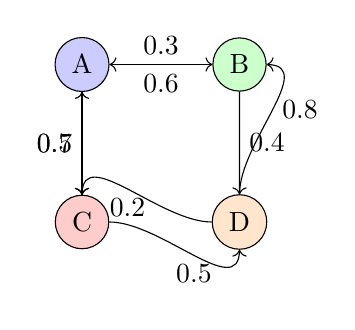
\begin{tikzpicture}[node distance=2cm]
    \node[circle, draw, fill=blue!20] (A) {A};
    \node[circle, draw, fill=green!20, right of=A] (B) {B};
    \node[circle, draw, fill=red!20, below of=A] (C) {C};
    \node[circle, draw, fill=orange!20, below of=B] (D) {D};
    
    \draw[->] (A) to[out=0,in=180] node[above] {0.3} (B);
    \draw[->] (A) to[out=270,in=90] node[left] {0.7} (C);
    \draw[->] (B) to[out=270,in=90] node[right] {0.4} (D);
    \draw[->] (B) to[out=180,in=0] node[below] {0.6} (A);
    \draw[->] (C) to[out=0,in=270] node[below] {0.5} (D);
    \draw[->] (C) to[out=90,in=270] node[left] {0.5} (A);
    \draw[->] (D) to[out=90,in=0] node[right] {0.8} (B);
    \draw[->] (D) to[out=180,in=90] node[below] {0.2} (C);
\end{tikzpicture}
\end{center}

\footnotesize
Markov chain with transition probabilities
\end{frame}

\begin{frame}{Heatmap Visualization}
\begin{center}
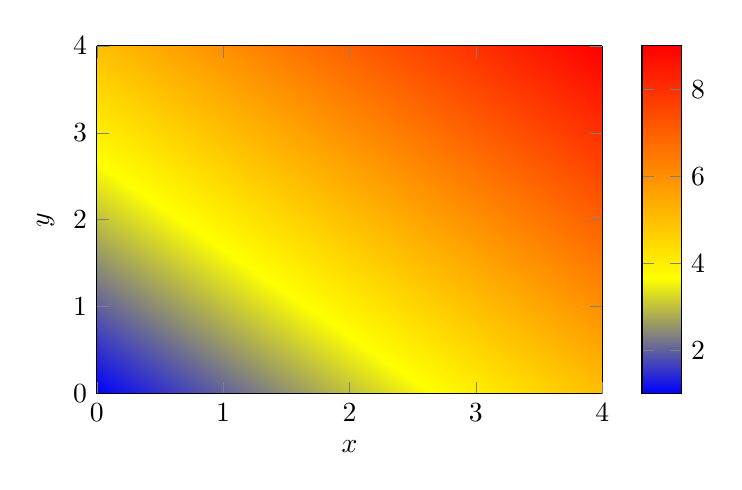
\begin{tikzpicture}
\begin{axis}[
    xlabel={$x$},
    ylabel={$y$},
    colorbar,
    width=8cm,
    height=6cm,
    view={0}{90}
]
\addplot3[surf, mesh/rows=5, mesh/cols=5, shader=interp] 
    coordinates {
        (0,0,1) (0,1,2) (0,2,3) (0,3,4) (0,4,5)
        (1,0,2) (1,1,3) (1,2,4) (1,3,5) (1,4,6)
        (2,0,3) (2,1,4) (2,2,5) (2,3,6) (2,4,7)
        (3,0,4) (3,1,5) (3,2,6) (3,3,7) (3,4,8)
        (4,0,5) (4,1,6) (4,2,7) (4,3,8) (4,4,9)
    };
\end{axis}
\end{tikzpicture}
\end{center}

\footnotesize
\texttt{\textbackslash addplot3[surf, mesh/rows=5, mesh/cols=5, shader=interp]}
\end{frame}

\begin{frame}{Polar Plot}
\begin{center}
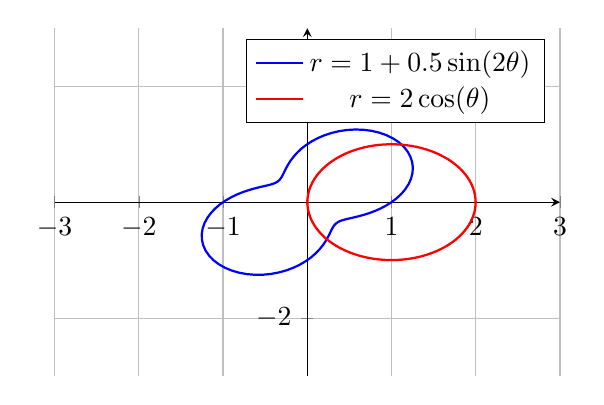
\begin{tikzpicture}
\begin{axis}[
    width=8cm,
    height=6cm,
    grid=both,
    legend pos=north east,
    axis lines=center,
    xmin=-3, xmax=3,
    ymin=-3, ymax=3
]
\addplot[thick, blue, domain=0:360, samples=100] ({cos(x)*(1 + 0.5*sin(2*x))}, {sin(x)*(1 + 0.5*sin(2*x))});
\addplot[thick, red, domain=0:360, samples=100] ({cos(x)*2*cos(x)}, {sin(x)*2*cos(x)});
\legend{$r = 1 + 0.5\sin(2\theta)$, $r = 2\cos(\theta)$}
\end{axis}
\end{tikzpicture}
\end{center}

\footnotesize
Polar plot converted to parametric form
\end{frame}

\begin{frame}{Error Bars}
\begin{center}
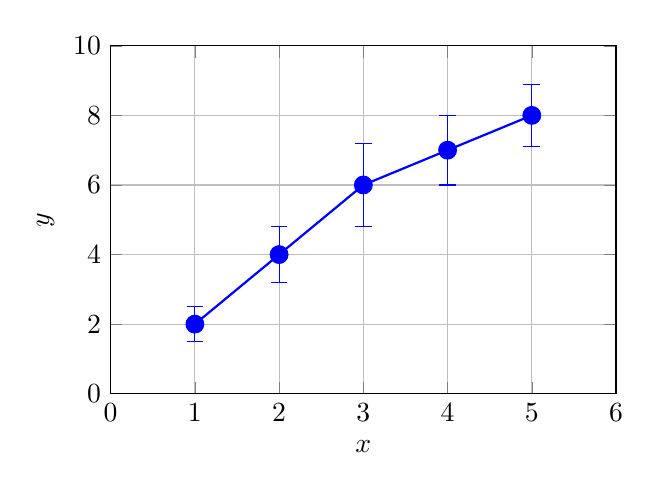
\begin{tikzpicture}
\begin{axis}[
    xlabel={$x$},
    ylabel={$y$},
    grid=both,
    xmin=0, xmax=6,
    ymin=0, ymax=10,
    width=8cm,
    height=6cm
]
\addplot[thick, blue, mark=*, mark size=3pt, error bars/.cd, y dir=both, y explicit] 
    coordinates {
        (1,2) +- (0,0.5)
        (2,4) +- (0,0.8)
        (3,6) +- (0,1.2)
        (4,7) +- (0,1.0)
        (5,8) +- (0,0.9)
    };
\end{axis}
\end{tikzpicture}
\end{center}

\footnotesize
\texttt{error bars/.cd, y dir=both, y explicit}
\end{frame}

\begin{frame}{Contour Plot}
\begin{center}
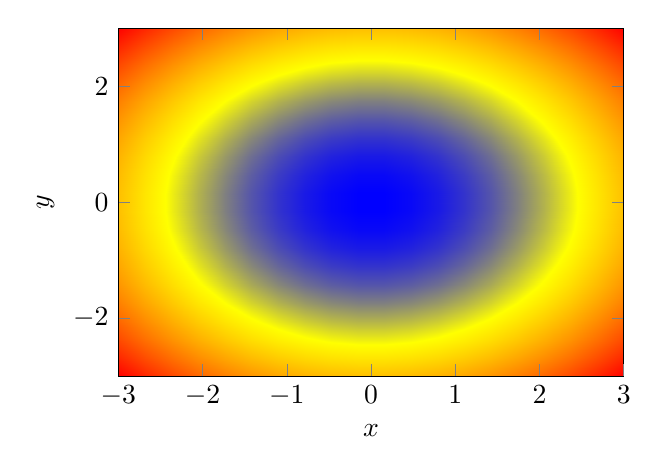
\begin{tikzpicture}
\begin{axis}[
    xlabel={$x$},
    ylabel={$y$},
    width=8cm,
    height=6cm,
    view={0}{90}
]
\addplot3[surf, domain=-3:3, domain y=-3:3, samples=20, shader=interp] {x^2 + y^2};
\end{axis}
\end{tikzpicture}
\end{center}

\footnotesize
\texttt{\textbackslash addplot3[surf, domain=-3:3, domain y=-3:3, samples=20, shader=interp] \{x\textasciicircum 2 + y\textasciicircum 2\};}
\end{frame}

\begin{frame}{Box Plot}
\begin{center}
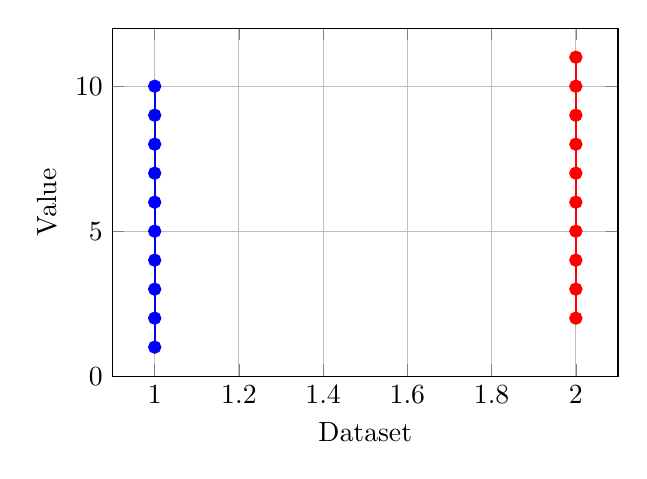
\begin{tikzpicture}
\begin{axis}[
    xlabel={Dataset},
    ylabel={Value},
    grid=both,
    width=8cm,
    height=6cm,
    ymin=0, ymax=12
]
% Simple box plot representation
\addplot[thick, blue, mark=*, mark size=2pt] coordinates {
    (1,1) (1,2) (1,3) (1,4) (1,5) (1,6) (1,7) (1,8) (1,9) (1,10)
};
\addplot[thick, red, mark=*, mark size=2pt] coordinates {
    (2,2) (2,3) (2,4) (2,5) (2,6) (2,7) (2,8) (2,9) (2,10) (2,11)
};
\end{axis}
\end{tikzpicture}
\end{center}

\footnotesize
Simplified box plot representation with scatter points
\end{frame}

\begin{frame}{Summary}
\begin{center}
\Large
\textbf{TikZ and PGFPlots Showcase Complete!}

\vspace{1cm}

\begin{itemize}
    \item Basic drawing and shapes
    \item Advanced plotting and visualization
    \item 3D graphics and animations
    \item Mathematical diagrams
    \item Data visualization
    \item And much more!
\end{itemize}

\vspace{1cm}

\footnotesize
This presentation demonstrates 50 different examples of TikZ and PGFPlots capabilities.
\end{center}
\end{frame}

\end{document}
